\section{Texture}

Dans le cadre de la détection de rupture, une autre caractéristique intéressante à exploiter est la texture des images. Différentes approches sont possibles pour représenter mathématiquement une texture. Pour ce projet, nous nous sommes intéressés à une approche statistique, avec la matrice de cooccurrence.

\subsection{Définition d'une texture}

En traitement d'image, on défini une texture comme étant \textit{une région spatiale d'une image présentant une organisation spatiale homogène des niveaux de luminance}. Une texture consiste en une reproduction de motifs de base dans l'espace et dans plusieurs directions. Ces motifs (ou primitives) sont organisés les uns par rapport aux autres de manière aléatoire.\\

D'après cette définition, on peut considérer une texture comme une structure à deux dimensions :

\begin{itemize}
    \item La première dimension représente les primitives formant la texture ;
    \item La seconde dimension représente l'organisation spatiale de ces primitives entre elles.
\end{itemize}

On recense deux types de texture, les macrotextures et les microtextures.

\begin{itemize}
    \item Une \textbf{macrotexture} est une texture structurée, pour laquelle on peut extraire facilement un motif de base et les lois d'assemblage des primitives entre elles. Par exemple, la texture d'un mur de briques est une macrotexture ;
    \item Une \textbf{microtexture} est une texture aléatoire, avec un aspect désorganisé, mais qui donne une impression visuelle relativement homogène. On peut prendre l'exemple d'une vue aérienne sur un champs.
\end{itemize}

Cependant, il est parfois difficile de classer une texture dans une catégorie ou l'autre. En fonction de la résolution de l'image ou du zoom effectué sur celle-ci, on va préférer classer la texture dans l'une ou l'autre des catégorie. On peut prendre l'exemple du sable, dans le cas où aucun zoom n'est effectué (\ref{noZoom}), il est tentant de classer cette texture en tant que macrotexture, alors que dans le cas où un zoom est effectué (\ref{Zoom}), il est plus probable de classer cette texture en tant que microtexture.

\begin{figure}
   \begin{minipage}[c]{.46\linewidth}
	  \centering
      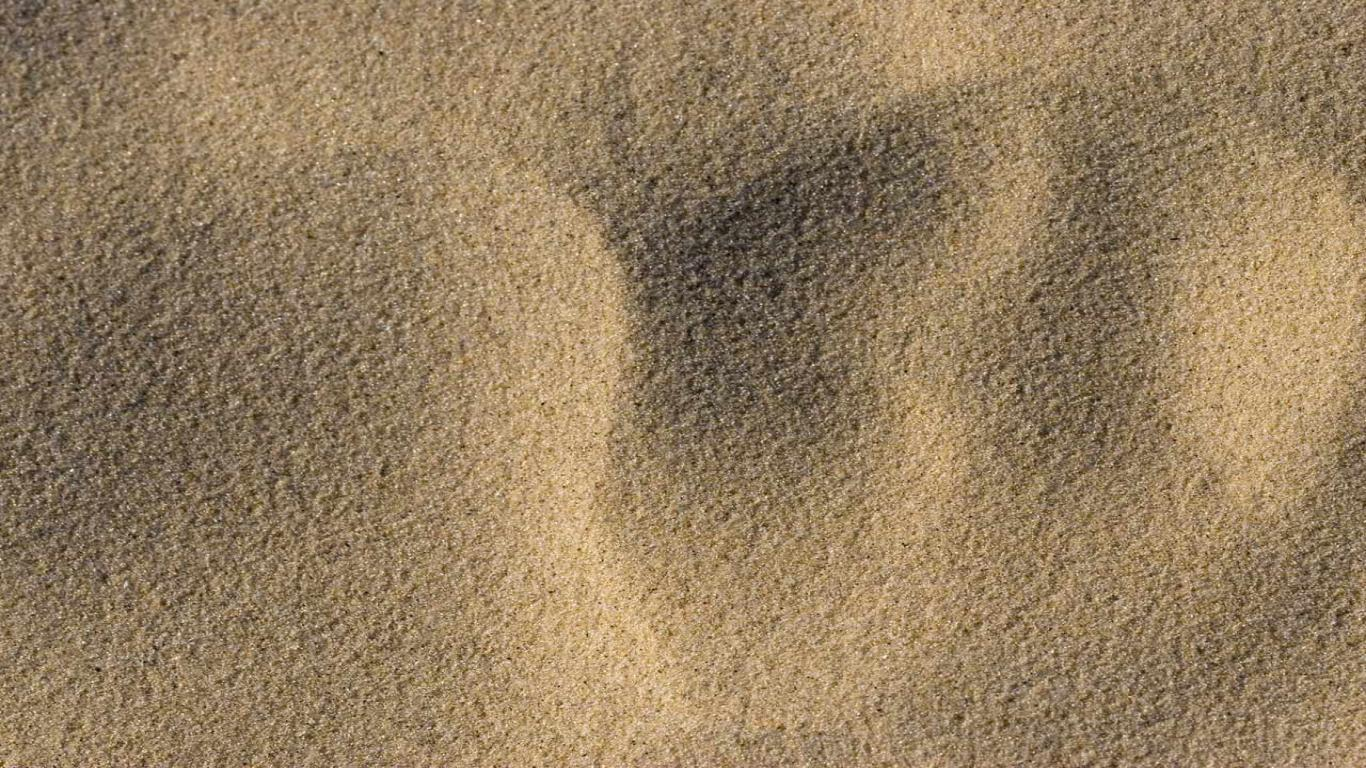
\includegraphics[scale=0.16]{images/sableNoZoom.jpg}
      \caption{\label{noZoom} Sable non zoomé}
   \end{minipage} \hfill
   \begin{minipage}[c]{.46\linewidth}
      \centering
      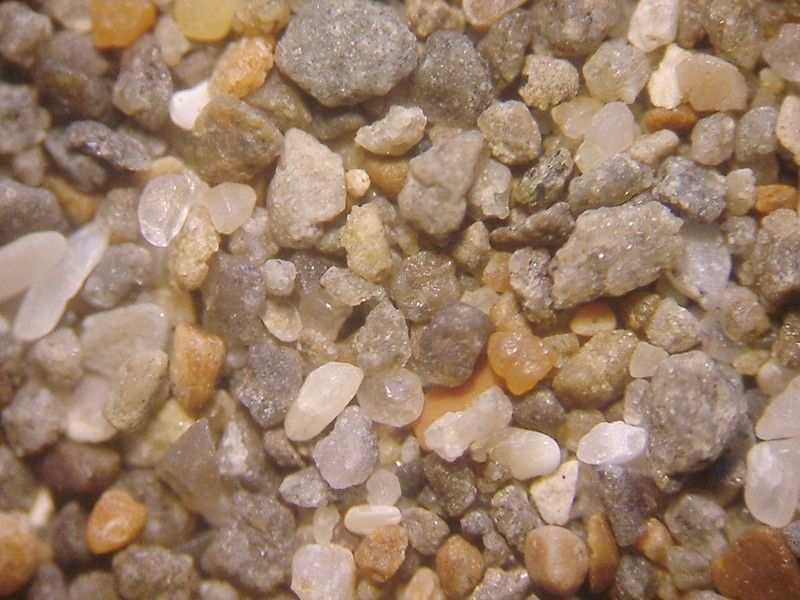
\includegraphics[scale=0.2]{images/sableZoom.jpg}
      \caption{\label{Zoom} Sable zoomé}
   \end{minipage}
\end{figure}

Il est important de retenir qu'une texture est une région d'une image pour laquelle il est possible de définir une fenêtre telle que pour toute translation de cette dernière, on retrouve le même motif. Une texture peut être décrite spatialement ou statistiquement. C'est cette dernière solution que nous tâcherons d'expliquer dans le cadre de ce projet, avec la matrice de cooccurrence.

\subsection{Matrice de cooccurrence}

En analyse de texture, cette méthode statistique donne des résultats relativement bons. Cette méthode consiste à compter le nombre de paires similaires de pixels ayant une distance $d$ entre eux. Cette méthode se base sur le niveau de gris des pixels, allant de 1 à 8. On prend également en compte la direction de la paire de pixels avec un angle $\theta$. Cette angle varie généralement entre $0$ et $180 degrés$. Les pixels d'une paire sont généralement séparés par une distance $d=1$ pixel.\\

Si on prend les paramètres suivants, $d=1, \theta = 0$, on obtient une paire de pixel comme suit :

\[
 \left \{
 \begin{array}{c @{=} c}
     pix_1 & (x_1, y_1) \\
     pix_2 & (x_2, y_2) \\
 \end{array}
 \right.
\]

avec $x_2 = x_1 + 1$ et $y_2 = y_1$.\\

Le pixel $pix_2$ est donc le voisin de droite du pixel $pix_1$. La matrice de cooccurrence est une matrice carrée $n\times n$, avec $n$ le niveau de gris (égale à 8 dans notre cas). Elle va recenser le nombre de pixels ayant un niveau de gris $n2$, situé à la droite d'un pixel dont le niveau de gris est $n1$. Les lignes de la matrice de cooccurrence représentent les pixels de référence et les colonnes, les pixels situés à droite du pixel de référence. Soit l'image $I$ dont les pixels ont les niveaux de gris suivants :

\[
 I = \begin{pmatrix}
     1 & 8 & 1 & 8 \\
     2 & 1 & 1 & 8 \\
     5 & 4 & 3 & 7 \\     
 \end{pmatrix}
\]

La matrice de cooccurrence de $I$ sera donc :

\[
 C = \begin{pmatrix}
     1 & 0 & 0 & 0 & 0 & 0 & 0 & 3 \\
     1 & 0 & 0 & 0 & 0 & 0 & 0 & 0 \\
     0 & 0 & 0 & 0 & 0 & 0 & 1 & 0 \\
     0 & 0 & 1 & 0 & 0 & 0 & 0 & 0 \\
     0 & 0 & 0 & 1 & 0 & 0 & 0 & 0 \\
     0 & 0 & 0 & 0 & 0 & 0 & 0 & 0 \\
     0 & 0 & 0 & 0 & 0 & 0 & 0 & 0 \\
     1 & 0 & 0 & 0 & 0 & 0 & 0 & 0 \\   
 \end{pmatrix}
\]

La valeur $C(1, 8) = 3$ signifie qu'il y a trois fois un pixel de niveau de gris $8$ à la droite d'un pixel de niveau de gris $1$.

\subsection{Détection de rupture et matrice de cooccurrence}

Voyons à présent en quoi la matrice de cooccurrence permet de détecter des ruptures dans une vidéo. Dans une vidéo, deux images consécutives seront relativement proches l'une de l'autre, excepté en cas de rupture. La matrice de cooccurrence va permettre d'obtenir une description de la texture de l'image. Entre deux image d'une même scène, la texture ne devrait pas changer et on devrait avoir deux matrices de cooccurrence très proches. Il faut rappeler que la texture d'une image est basé sur la répétition de motifs, et donc, dans une scène, on devrait retrouver les mêmes motifs. Dans notre cas, dans une même scène, les niveaux de gris ne devraient pas énormément évoluer d'une image à l'autre.\\

La méthode des matrices de cooccurrence possède certains avantages, mais également quelques inconvénients.

\subsection{Avantages}

Les avantages de cette méthode sont les suivants :

\begin{itemize}
	\item Simple à mettre en oeuvre ;
	\item Relativement robuste aux mouvements.
\end{itemize}

\subsection{Inconvénients}

Les inconvénients de cette méthode sont les suivants :

\begin{itemize}
	\item Basée sur les niveaux de gris, donc peu robuste aux transitions avec un effet de fondu ;
	\item Peu robuste aux changement d'intensité d'une couleur (comme le bleu du ciel) ;
	\item Peu robuste à l'apparition de nouveaux objets sur une scène.
\end{itemize}
